\documentclass{report}
\usepackage{graphicx, tikz-cd, float, titlepic, booktabs} % Required for inserting images
\usepackage{amsmath, amssymb, amsthm, amsfonts, siunitx, physics, gensymb}
\AtBeginDocument{\RenewCommandCopy\qty\SI}
\usepackage[version=4]{mhchem}
\usepackage[most,many,breakable]{tcolorbox}
\usepackage{xcolor, fancyhdr, varwidth}
\usepackage[Glenn]{fncychap}
%Options: Sonny, Lenny, Glenn, Conny, Rejne, Bjarne, Bjornstrup
\usepackage{hyperref, cleveref}
\usepackage{icomma, enumitem} %comma as decimal and continue enumerate with [resume]
%%%%%%%%%%%%%%%%%%%%%%%%%%%%%%
% SELF MADE COLORS
%%%%%%%%%%%%%%%%%%%%%%%%%%%%%%
\definecolor{myg}{RGB}{56, 140, 70}
\definecolor{myb}{RGB}{45, 111, 177}
\definecolor{myr}{RGB}{199, 68, 64}
\definecolor{mytheorembg}{HTML}{F2F2F9}
\definecolor{mytheoremfr}{HTML}{00007B}
\definecolor{mylenmabg}{HTML}{FFFAF8}
\definecolor{mylenmafr}{HTML}{983b0f}
\definecolor{mypropbg}{HTML}{f2fbfc}
\definecolor{mypropfr}{HTML}{191971}
\definecolor{myexamplebg}{HTML}{F2FBF8}
\definecolor{myexamplefr}{HTML}{88D6D1}
\definecolor{myexampleti}{HTML}{2A7F7F}
\definecolor{mydefinitbg}{HTML}{E5E5FF}
\definecolor{mydefinitfr}{HTML}{3F3FA3}
\definecolor{notesgreen}{RGB}{0,162,0}
\definecolor{myp}{RGB}{197, 92, 212}
\definecolor{mygr}{HTML}{2C3338}
\definecolor{myred}{RGB}{127,0,0}
\definecolor{myyellow}{RGB}{169,121,69}
\definecolor{myexercisebg}{HTML}{F2FBF8}
\definecolor{myexercisefg}{HTML}{88D6D1}
%%%%%%%%%%%%%%%%%%%%%%%%%%%%%%%%%%%%%%%%%%%%%%%%%%%%%%%%%%%%%%%%%%%%%%
% Box environments for theorems and problems
%%%%%%%%%%%%%%%%%%%%%%%%%%%%%%%%%%%%%%%%%%%%%%%%%%%%%%%%%%%%%%%%%%%%%
\setlength{\parindent}{1cm}
%================================
% Question BOX
%================================
\makeatletter
\newtcbtheorem{question}{Opgave}{enhanced,
	breakable,
	colback=white,
	colframe=myb!80!black,
	attach boxed title to top left={yshift*=-\tcboxedtitleheight},
	fonttitle=\bfseries,
	title={#2},
	boxed title size=title,
	boxed title style={%
			sharp corners,
			rounded corners=northwest,
			colback=tcbcolframe,
			boxrule=0pt,
		},
	underlay boxed title={%
			\path[fill=tcbcolframe] (title.south west)--(title.south east)
			to[out=0, in=180] ([xshift=5mm]title.east)--
			(title.center-|frame.east)
			[rounded corners=\kvtcb@arc] |-
			(frame.north) -| cycle;
		},
	#1
}{def}
\makeatother
%================================
% DEFINITION BOX
%================================

\newtcbtheorem[]{Definition}{Definition}{enhanced,
	before skip=2mm,after skip=2mm, colback=red!5,colframe=red!80!black,boxrule=0.5mm,
	attach boxed title to top left={xshift=1cm,yshift*=1mm-\tcboxedtitleheight}, varwidth boxed title*=-3cm,
	boxed title style={frame code={
					\path[fill=tcbcolback]
					([yshift=-1mm,xshift=-1mm]frame.north west)
					arc[start angle=0,end angle=180,radius=1mm]
					([yshift=-1mm,xshift=1mm]frame.north east)
					arc[start angle=180,end angle=0,radius=1mm];
					\path[left color=tcbcolback!60!black,right color=tcbcolback!60!black,
						middle color=tcbcolback!80!black]
					([xshift=-2mm]frame.north west) -- ([xshift=2mm]frame.north east)
					[rounded corners=1mm]-- ([xshift=1mm,yshift=-1mm]frame.north east)
					-- (frame.south east) -- (frame.south west)
					-- ([xshift=-1mm,yshift=-1mm]frame.north west)
					[sharp corners]-- cycle;
				},interior engine=empty,
		},
	fonttitle=\bfseries,
	title={#2},#1}{def}
\newtcbtheorem[]{definition}{Definition}{enhanced,
	before skip=2mm,after skip=2mm, colback=red!5,colframe=red!80!black,boxrule=0.5mm,
	attach boxed title to top left={xshift=1cm,yshift*=1mm-\tcboxedtitleheight}, varwidth boxed title*=-3cm,
	boxed title style={frame code={
					\path[fill=tcbcolback]
					([yshift=-1mm,xshift=-1mm]frame.north west)
					arc[start angle=0,end angle=180,radius=1mm]
					([yshift=-1mm,xshift=1mm]frame.north east)
					arc[start angle=180,end angle=0,radius=1mm];
					\path[left color=tcbcolback!60!black,right color=tcbcolback!60!black,
						middle color=tcbcolback!80!black]
					([xshift=-2mm]frame.north west) -- ([xshift=2mm]frame.north east)
					[rounded corners=1mm]-- ([xshift=1mm,yshift=-1mm]frame.north east)
					-- (frame.south east) -- (frame.south west)
					-- ([xshift=-1mm,yshift=-1mm]frame.north west)
					[sharp corners]-- cycle;
				},interior engine=empty,
		},
	fonttitle=\bfseries,
	title={#2},#1}{def}

\newtcbtheorem{theo}%
    {Theorem}{}{theorem}
\newtcolorbox{prob}[1]{colback=red!5!white,colframe=red!50!black,fonttitle=\bfseries,title={#1}}
%================================
% NOTE BOX
%================================

\usetikzlibrary{arrows,calc,shadows.blur}
\tcbuselibrary{skins}
\newtcolorbox{note}[1][]{%
	enhanced jigsaw,
	colback=gray!20!white,%
	colframe=gray!80!black,
	size=small,
	boxrule=1pt,
	title=\textbf{Note:},
	halign title=flush center,
	coltitle=black,
	breakable,
	drop shadow=black!50!white,
	attach boxed title to top left={xshift=1cm,yshift=-\tcboxedtitleheight/2,yshifttext=-\tcboxedtitleheight/2},
	minipage boxed title=1.5cm,
	boxed title style={%
			colback=white,
			size=fbox,
			boxrule=1pt,
			boxsep=2pt,
			underlay={%
					\coordinate (dotA) at ($(interior.west) + (-0.5pt,0)$);
					\coordinate (dotB) at ($(interior.east) + (0.5pt,0)$);
					\begin{scope}
						\clip (interior.north west) rectangle ([xshift=3ex]interior.east);
						\filldraw [white, blur shadow={shadow opacity=60, shadow yshift=-.75ex}, rounded corners=2pt] (interior.north west) rectangle (interior.south east);
					\end{scope}
					\begin{scope}[gray!80!black]
						\fill (dotA) circle (2pt);
						\fill (dotB) circle (2pt);
					\end{scope}
				},
		},
	#1,
}

%%%%%%%%%%%%%%%%%%%%%%%%%%%%%%%%%%%%%%%%%%%%%%%%%%%%%%%%%%%%%%%%%
% SELF MADE COMMANDS
%%%%%%%%%%%%%%%%%%%%%%%%%%%%%%
\newcommand{\sol}{\setlength{\parindent}{0cm}\textbf{\textit{Løsning:}}\setlength{\parindent}{1cm}}
%%%%%%%%%%%%%%%%%%%%%%%%%%%%%%%%%
\usepackage[tmargin=2cm,rmargin=1in,lmargin=1in,margin=0.85in,bmargin=2cm,footskip=.2in]{geometry}\pagestyle{fancy}
\lhead{Minrui Kevin Zhou 2.b}
\rhead{Matematikaflevering 19}

\title{Aflevering 19\\
{\Large \textbf{2.b mat A}}}
\author{Kevin Zhou}
\date{November 2023}

\begin{document}
\maketitle
\begin{question}{}{}
Funktionen $f:\mathbb{R} \to \mathbb{R}$ er bestemt ved
\[
  f(x)=x^4-14x^2+24x.
\] 
\begin{itemize}
  \item[a.] Bestem monotoniforholdene for $f$.
  \item[b.] Bestem minimum for $f$.
\end{itemize}
\end{question}
\sol \\ 
\textbf{a.} Vi bestemmer først den afledede funktion.
\[
f'(x)=4x^3-28x+24
\] 
Vi kan da finde løsningerne til ligningen $f'(x)=0$.
\[
4x^3-28x+24=0 \implies x=-3 \lor x=1 \lor x=2
\] 
Vi bestemmer nu den dobbeltafledede funktion.
\[
f''(x)=\dv{x} (4x^3-28x+24) = 12x^2 - 28
\] 
Siden 
\begin{equation*}
\begin{split}
f''(-3)&=80>0\\ 
  f''(1)&=-16<0\\ 
  f''(2)&=20>0
\end{split}
\end{equation*}
så må $-3$ være et lokalt minimumssted, $1$ være et lokalt maksimumssted og $2$ være et lokalt minimumssted.
Ud fra dette kan vi nemt bestemme monotoniforholdene for $f$. 
\begin{equation*}
\begin{split}
  &f \text{ er aftagende på } (-\infty ;-3]\\
  &f \text{ er voksende på } [-3,1]\\ 
  &f \text{ er aftagende på } [1;2]\\
  &f \text{ er voksende på } [2;\infty)
\end{split}
\end{equation*}
\textbf{b.}
Fra delopgave \textbf{a.} ved vi, at $-3$ og $2$ er lokale minimumssteder.
Vi kan da nemt regne disse lokale minima.
\begin{equation*}
\begin{split}
  f(-3)&= -117\\ 
  f(2)&= 8
\end{split}
\end{equation*}
Altså er $-117$ det globale minimum.

\begin{question}{}{}
Funktionen $f:[0;12]\to \mathbb{R}$ er givet ved 
\[
f(x)= 0,5x \cdot \sqrt{144-x^2} 
\] 
\begin{itemize}
  \item[a.] Tegn grafen for $f$.
  \item[b.] Bestem maksimum for $f$.
\end{itemize}
\end{question}
\sol \\ 
\textbf{a.}
Grafen for $f$ kan ses i \cref{fig:opg2}.
\begin{figure}[H]
\begin{center}
  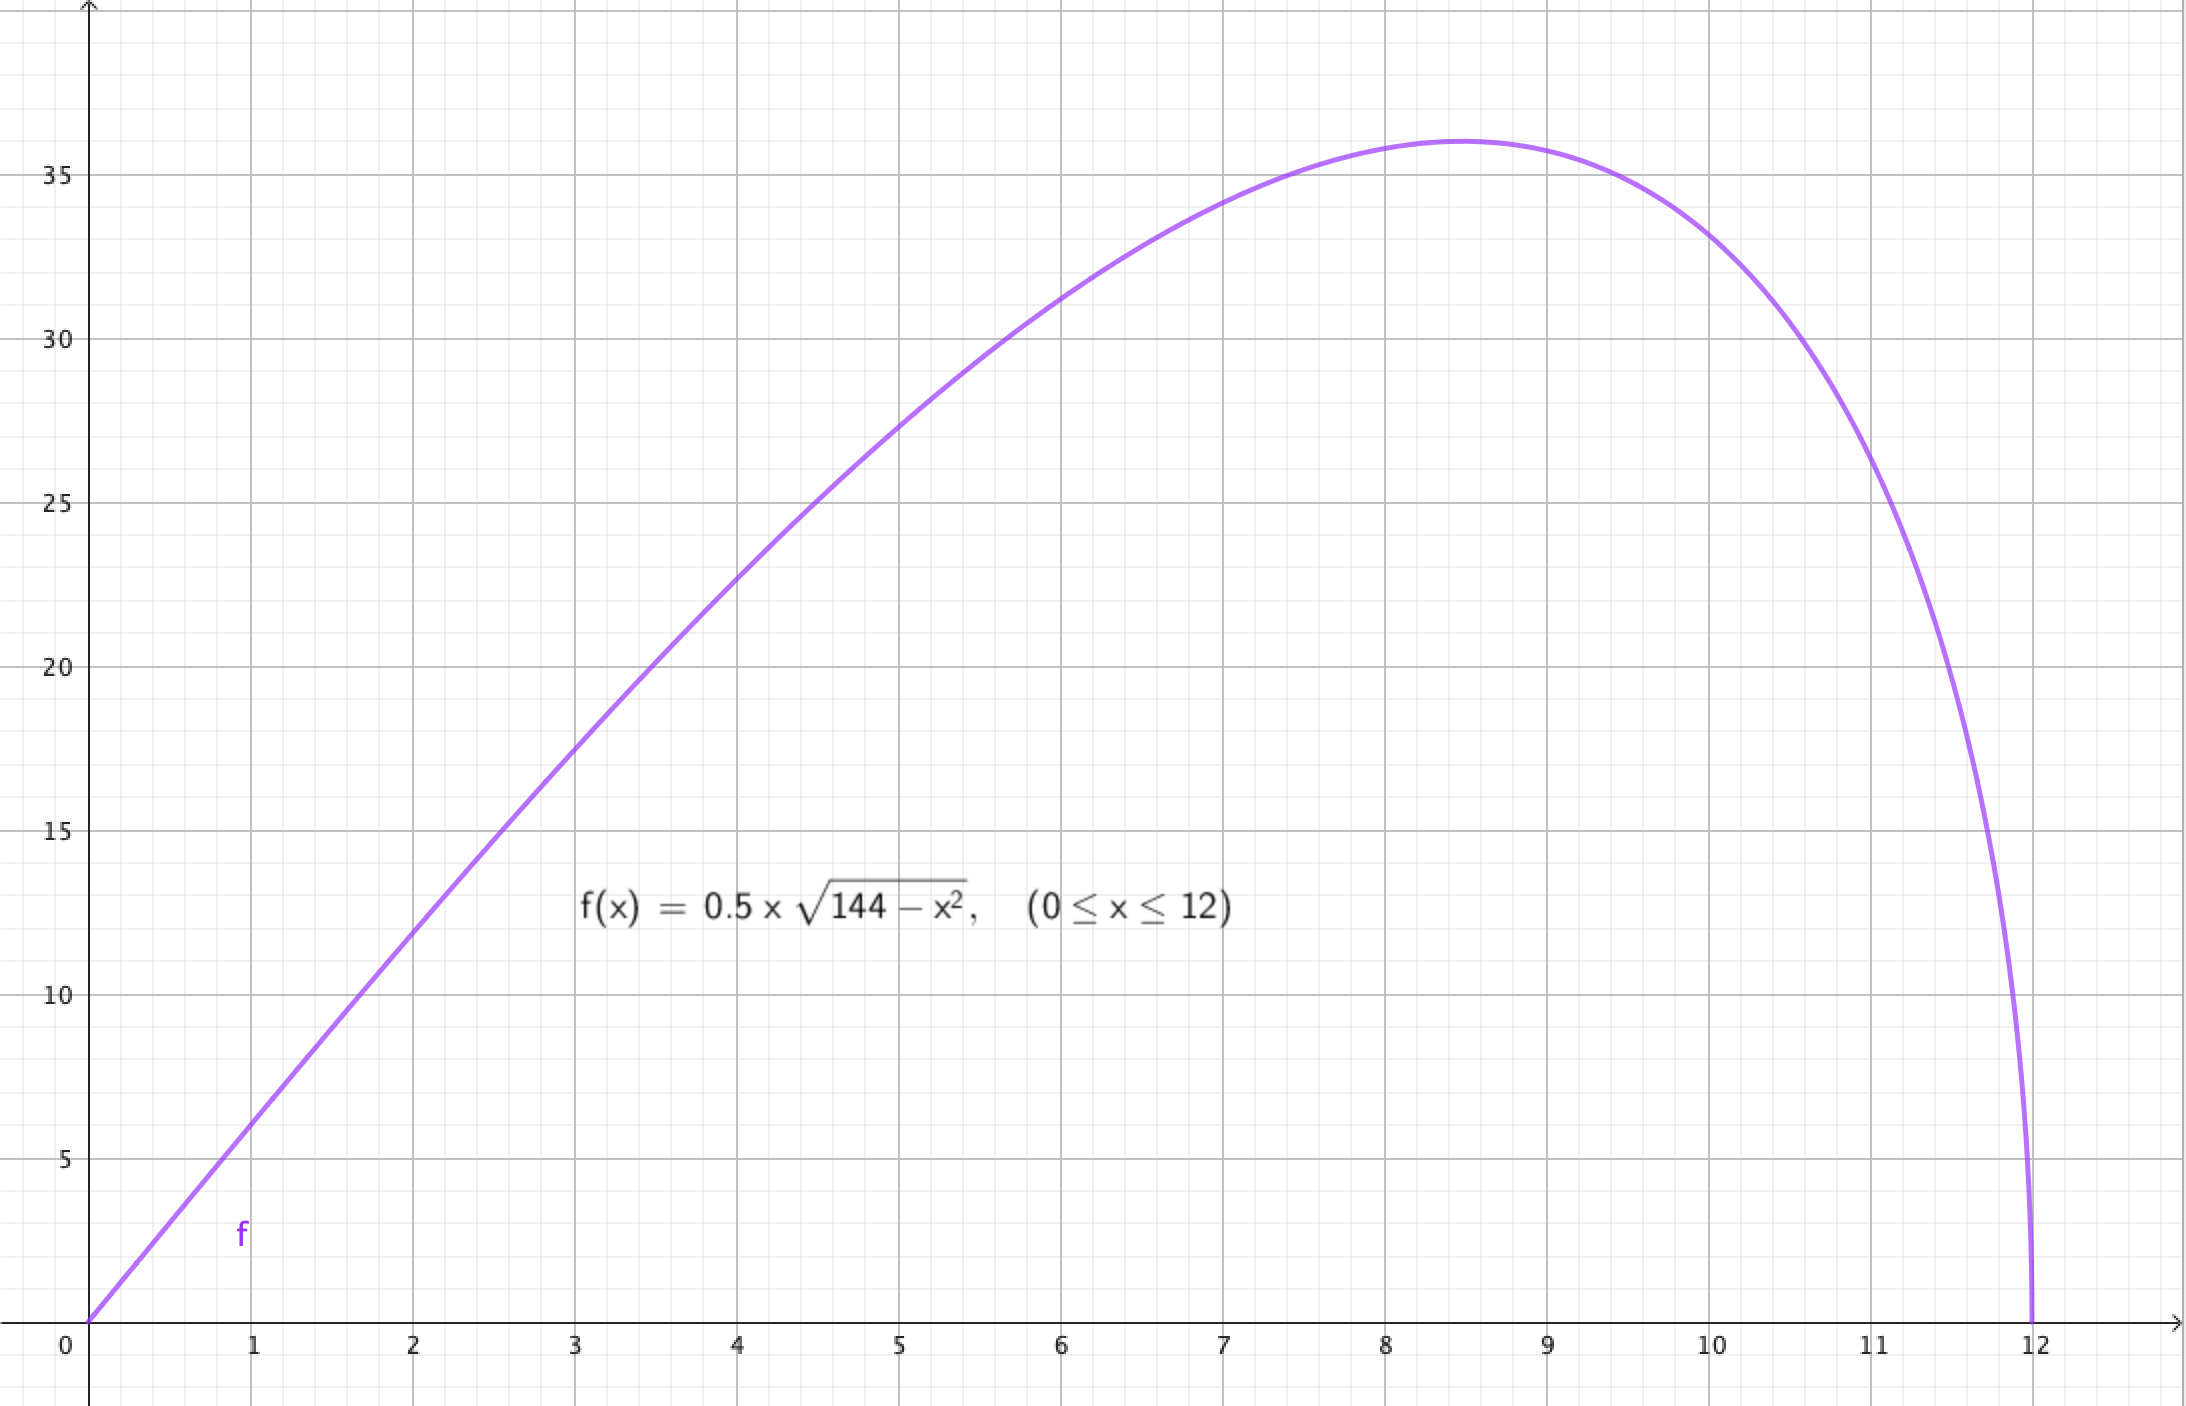
\includegraphics[width=\textwidth]{opg2.png}
\end{center}
\caption{Grafen for $f$}
\label{fig:opg2}
\end{figure}
\noindent \textbf{b.}
Den afledede funktion regnes.
\[
f'(x)=0,5\cdot \left(\sqrt{144-x^2} + x \cdot \left(-\frac{x}{\sqrt{144-x^2} }\right) \right)
=\frac{72-x^2}{\sqrt{144-x^2} }
\] 
Vi finder nu løsningerne til $f'(x)=0$ via CAS.
\[
\frac{72-x^2}{\sqrt{144-x^2} }=0 \implies x=-6 \sqrt{2} \lor x=6 \sqrt{2} 
\] 
Det er dog kun en af disse, som tilhører definitionsmængden for $f$:
\begin{equation*}
\begin{split}
  -6 \sqrt{2} &\not\in Dm(f)\\ 
  6 \sqrt{2} &\in Dm(f)
\end{split}
\end{equation*}
Altså vil det sige, at
\[
f'(x)=0 \implies x=6 \sqrt{2} 
\] 
Vi regner nu den dobbeltafledede funktion af $f$ med lommeregneren. 
\[
f''(x)=\dv{x} (\frac{72-x^2}{\sqrt{144-x^2} })
=\frac{x\left(x^2-216\right)}{\left(144-x^2\right)^{3/2}}
\] 
Med lommeregneren får vi, at
\[
f''(x)=-2<0
\] 
Derfor må $6 \sqrt{2} $ være det globale maksimumssted.
Det globale maksimum må være
\[
f(6 \sqrt{2} )= 36
\] 
\begin{question}{}{}
I en model beskrives udviklingen i det årlige antal nedlagte råvild i Danmark med 
\[
  f(x)= \frac{150000}{1+2,6\cdot e^{-0,1x}},
\] 
  hvor $f(x)$ angiver det årlige antal nedlagte råvild til tidspunktet $x$ år efter 1980
\begin{itemize}
  \item[a.] Benyt modellen til at bestemme det årstal, hvor det årlige antal nedlagte råvildt var 120000.
  \item[b.] Bestem væksthastigheden for det årlige antal nedlagte råvildt til tidspunktet $x=40$.
\end{itemize}
\end{question}
\sol \\ 
\textbf{a.} Årstallet finder vi ved at løse den nedenstående opstillede ligning.
\begin{equation*}
\begin{split}
  f(x)= 120000 &\implies \frac{150000}{1+2,6\cdot e^{-0,1x}}=120000 \\ 
  &\iff -0,1x = \ln(\frac{30000}{2,6\cdot 120000}) \\ 
  &\iff x=-10\cdot \ln(\frac{30000}{2,6\cdot 120000}) \approx 23,42
\end{split}
\end{equation*}
Årstallet kan nu bestemmes.
\[
1980 + 23,42 = 2003,42
\] 
Vi runder her ned. Altså da det årlige antal nedlagte råvildt var 120000 var årstallet 2003. \\[1ex]
\textbf{b.} Vi finder først den afledede funktion via kædereglen.
\begin{equation*}
\begin{split}
  f'(x)&=150000 \left(\dv{x} \left(\frac{1}{1+2,6\cdot e^{-0,1x}}\right)\right) \\ 
  &=150000 \cdot \left(-\frac{1}{\left(1+2,6 \cdot e^{-0,1x}\right)^2}\right)\cdot (-0,26 e^{-0,1x})\\ 
  &= \frac{39000}{(1+2,6\cdot e^{-0,1x})^2}
\end{split}
\end{equation*}
Vi kan nu bestemme væksthastigheden for det årlige antal nedlagte råvildt via en lommeregner.
\[
f'(40)\approx 650,846
\] 
Altså vokser det årlige antal nedlagte råvildt til tidspunktet $x=40$ ifølge modellen 650,846 råvildt per år. 
\end{document}
